% Created by tikzDevice version 0.12.3.1 on 2022-09-02 10:37:00
% !TEX encoding = UTF-8 Unicode
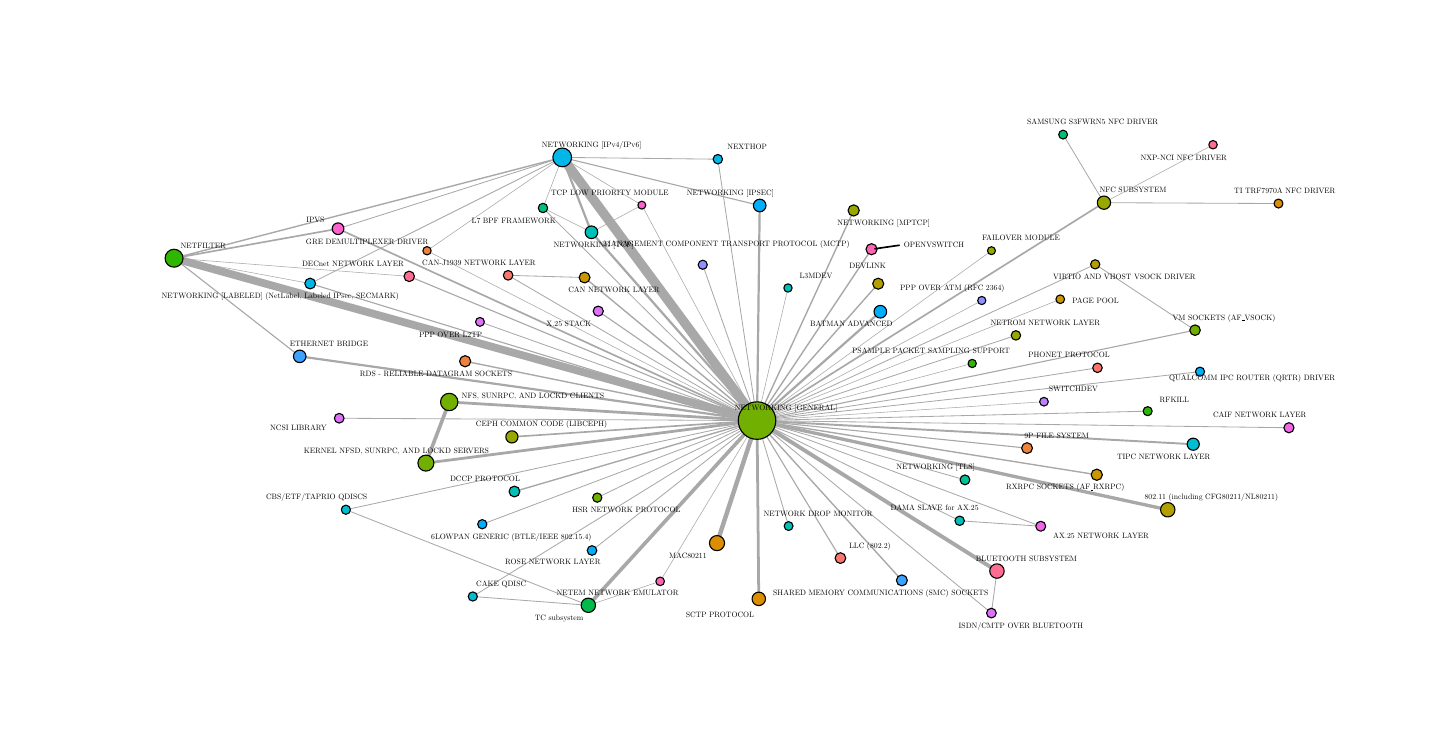
\begin{tikzpicture}[x=1pt,y=1pt]
\definecolor{fillColor}{RGB}{255,255,255}
\path[use as bounding box,fill=fillColor,fill opacity=0.00] (0,0) rectangle (505.89,252.94);
\begin{scope}
\path[clip] (  0.00,  0.00) rectangle (505.89,252.94);
\definecolor{fillColor}{RGB}{255,255,255}

\path[fill=fillColor] (  0.00,  0.00) rectangle (505.89,252.94);
\end{scope}
\begin{scope}
\path[clip] ( 32.75, 32.75) rectangle (475.89,222.94);
\definecolor{drawColor}{gray}{0.66}

\path[draw=drawColor,line width= 0.3pt,line join=round] (164.27, 73.51) -- (263.55,110.96);

\path[draw=drawColor,line width= 1.2pt,line join=round] (411.97, 78.74) -- (263.55,110.96);

\path[draw=drawColor,line width= 0.4pt,line join=round] (361.12,101.01) -- (263.55,110.96);

\path[draw=drawColor,line width= 0.3pt,line join=round] (366.07, 72.78) -- (336.77, 74.76);

\path[draw=drawColor,line width= 0.3pt,line join=round] (366.07, 72.78) -- (263.55,110.96);

\path[draw=drawColor,line width= 0.8pt,line join=round] (308.11,150.29) -- (263.55,110.96);

\path[draw=drawColor,line width= 0.3pt,line join=round] (350.25, 56.59) -- (348.24, 41.40);

\path[draw=drawColor,line width= 1.4pt,line join=round] (350.25, 56.59) -- (263.55,110.96);

\path[draw=drawColor,line width= 0.3pt,line join=round] (455.75,108.37) -- (263.55,110.96);

\path[draw=drawColor,line width= 0.3pt,line join=round] (160.84, 47.40) -- (263.55,110.96);

\path[draw=drawColor,line width= 0.3pt,line join=round] (160.84, 47.40) -- (202.59, 44.22);

\path[draw=drawColor,line width= 0.3pt,line join=round] (201.23,162.65) -- (173.61,163.45);

\path[draw=drawColor,line width= 0.5pt,line join=round] (201.23,162.65) -- (263.55,110.96);

\path[draw=drawColor,line width= 0.3pt,line join=round] (173.61,163.45) -- (263.55,110.96);

\path[draw=drawColor,line width= 0.3pt,line join=round] (114.98, 78.75) -- (263.55,110.96);

\path[draw=drawColor,line width= 0.3pt,line join=round] (114.98, 78.75) -- (202.59, 44.22);

\path[draw=drawColor,line width= 0.6pt,line join=round] (174.98,105.07) -- (263.55,110.96);

\path[draw=drawColor,line width= 0.3pt,line join=round] (336.77, 74.76) -- (263.55,110.96);

\path[draw=drawColor,line width= 0.5pt,line join=round] (175.89, 85.33) -- (263.55,110.96);

\path[draw=drawColor,line width= 0.2pt,line join=round] (137.87,163.07) -- ( 52.89,169.63);

\path[draw=drawColor,line width= 0.4pt,line join=round] (137.87,163.07) -- (263.55,110.96);

\path[draw=drawColor,line width= 0.5pt,line join=round] (307.34,160.42) -- (263.55,110.96);

\path[draw=drawColor,line width= 0.4pt,line join=round] ( 98.30,134.17) -- ( 52.89,169.63);

\path[draw=drawColor,line width= 0.8pt,line join=round] ( 98.30,134.17) -- (263.55,110.96);

\path[draw=drawColor,line width= 0.2pt,line join=round] (348.26,172.35) -- (263.55,110.96);

\path[draw=drawColor,line width= 0.2pt,line join=round] (144.30,172.33) -- (263.55,110.96);

\path[draw=drawColor,line width= 0.2pt,line join=round] (144.30,172.33) -- (193.16,206.06);

\path[draw=drawColor,line width= 0.3pt,line join=round] (205.82, 83.12) -- (263.55,110.96);

\path[draw=drawColor,line width= 0.6pt,line join=round] (112.16,180.29) -- ( 52.89,169.63);

\path[draw=drawColor,line width= 0.6pt,line join=round] (112.16,180.29) -- (263.55,110.96);

\path[draw=drawColor,line width= 0.3pt,line join=round] (112.16,180.29) -- (193.16,206.06);

\path[draw=drawColor,line width= 0.3pt,line join=round] (348.24, 41.40) -- (263.55,110.96);

\path[draw=drawColor,line width= 1.0pt,line join=round] (143.90, 95.60) -- (263.55,110.96);

\path[draw=drawColor,line width= 1.3pt,line join=round] (143.90, 95.60) -- (152.33,117.68);

\path[draw=drawColor,line width= 0.2pt,line join=round] (274.73,158.88) -- (263.55,110.96);

\path[draw=drawColor,line width= 0.3pt,line join=round] (186.20,187.78) -- (263.55,110.96);

\path[draw=drawColor,line width= 0.2pt,line join=round] (186.20,187.78) -- (193.16,206.06);

\path[draw=drawColor,line width= 0.2pt,line join=round] (186.20,187.78) -- (203.71,179.01);

\path[draw=drawColor,line width= 0.4pt,line join=round] (293.68, 61.27) -- (263.55,110.96);

\path[draw=drawColor,line width= 1.6pt,line join=round] (249.09, 66.69) -- (263.55,110.96);

\path[draw=drawColor,line width= 0.3pt,line join=round] (243.93,167.27) -- (263.55,110.96);

\path[draw=drawColor,line width= 0.3pt,line join=round] (112.57,111.81) -- (263.55,110.96);

\path[draw=drawColor,line width= 0.2pt,line join=round] (228.54, 52.87) -- (263.55,110.96);

\path[draw=drawColor,line width= 0.2pt,line join=round] (228.54, 52.87) -- (202.59, 44.22);

\path[draw=drawColor,line width= 2.8pt,line join=round] ( 52.89,169.63) -- (263.55,110.96);

\path[draw=drawColor,line width= 0.5pt,line join=round] ( 52.89,169.63) -- (193.16,206.06);

\path[draw=drawColor,line width= 0.2pt,line join=round] ( 52.89,169.63) -- (102.08,160.48);

\path[draw=drawColor,line width= 0.3pt,line join=round] (357.10,141.74) -- (263.55,110.96);

\path[draw=drawColor,line width= 0.3pt,line join=round] (274.96, 72.85) -- (263.55,110.96);

\path[draw=drawColor,line width= 0.8pt,line join=round] (263.55,110.96) -- (264.52,188.68);

\path[draw=drawColor,line width= 3.4pt,line join=round] (263.55,110.96) -- (193.16,206.06);

\path[draw=drawColor,line width= 0.4pt,line join=round] (263.55,110.96) -- (102.08,160.48);

\path[draw=drawColor,line width= 0.5pt,line join=round] (263.55,110.96) -- (298.47,186.89);

\path[draw=drawColor,line width= 0.8pt,line join=round] (263.55,110.96) -- (203.71,179.01);

\path[draw=drawColor,line width= 0.3pt,line join=round] (263.55,110.96) -- (338.69, 89.54);

\path[draw=drawColor,line width= 0.3pt,line join=round] (263.55,110.96) -- (249.39,205.41);

\path[draw=drawColor,line width= 0.6pt,line join=round] (263.55,110.96) -- (388.91,189.70);

\path[draw=drawColor,line width= 1.0pt,line join=round] (263.55,110.96) -- (152.33,117.68);

\path[draw=drawColor,line width= 0.5pt,line join=round] (263.55,110.96) -- (304.93,172.88);

\path[draw=drawColor,line width= 0.2pt,line join=round] (263.55,110.96) -- (373.12,154.80);

\path[draw=drawColor,line width= 0.3pt,line join=round] (263.55,110.96) -- (386.57,130.03);

\path[draw=drawColor,line width= 0.2pt,line join=round] (263.55,110.96) -- (344.76,154.34);

\path[draw=drawColor,line width= 0.3pt,line join=round] (263.55,110.96) -- (163.43,146.63);

\path[draw=drawColor,line width= 0.2pt,line join=round] (263.55,110.96) -- (341.30,131.59);

\path[draw=drawColor,line width= 0.3pt,line join=round] (263.55,110.96) -- (423.62,128.64);

\path[draw=drawColor,line width= 0.5pt,line join=round] (263.55,110.96) -- (158.08,132.40);

\path[draw=drawColor,line width= 0.3pt,line join=round] (263.55,110.96) -- (404.70,114.36);

\path[draw=drawColor,line width= 0.3pt,line join=round] (263.55,110.96) -- (203.92, 64.02);

\path[draw=drawColor,line width= 0.5pt,line join=round] (263.55,110.96) -- (386.31, 91.39);

\path[draw=drawColor,line width= 1.0pt,line join=round] (263.55,110.96) -- (264.18, 46.54);

\path[draw=drawColor,line width= 0.5pt,line join=round] (263.55,110.96) -- (315.89, 53.22);

\path[draw=drawColor,line width= 0.2pt,line join=round] (263.55,110.96) -- (367.23,117.78);

\path[draw=drawColor,line width= 1.3pt,line join=round] (263.55,110.96) -- (202.59, 44.22);

\path[draw=drawColor,line width= 0.2pt,line join=round] (263.55,110.96) -- (221.92,188.81);

\path[draw=drawColor,line width= 0.7pt,line join=round] (263.55,110.96) -- (421.17,102.42);

\path[draw=drawColor,line width= 0.3pt,line join=round] (263.55,110.96) -- (385.75,167.41);

\path[draw=drawColor,line width= 0.4pt,line join=round] (263.55,110.96) -- (421.82,143.63);

\path[draw=drawColor,line width= 0.4pt,line join=round] (263.55,110.96) -- (206.18,150.50);

\path[draw=drawColor,line width= 0.4pt,line join=round] (264.52,188.68) -- (193.16,206.06);

\path[draw=drawColor,line width= 0.3pt,line join=round] (193.16,206.06) -- (102.08,160.48);

\path[draw=drawColor,line width= 0.8pt,line join=round] (193.16,206.06) -- (203.71,179.01);

\path[draw=drawColor,line width= 0.3pt,line join=round] (193.16,206.06) -- (249.39,205.41);

\path[draw=drawColor,line width= 0.2pt,line join=round] (193.16,206.06) -- (221.92,188.81);

\path[draw=drawColor,line width= 0.2pt,line join=round] (203.71,179.01) -- (221.92,188.81);

\path[draw=drawColor,line width= 0.2pt,line join=round] (388.91,189.70) -- (428.32,210.64);

\path[draw=drawColor,line width= 0.3pt,line join=round] (388.91,189.70) -- (374.15,214.30);

\path[draw=drawColor,line width= 0.3pt,line join=round] (388.91,189.70) -- (451.98,189.39);

\path[draw=drawColor,line width= 0.3pt,line join=round] (385.75,167.41) -- (421.82,143.63);
\definecolor{drawColor}{RGB}{0,0,0}
\definecolor{fillColor}{RGB}{0,174,250}

\path[draw=drawColor,line width= 0.4pt,line join=round,line cap=round,fill=fillColor] (164.27, 73.51) circle (  1.67);
\definecolor{fillColor}{RGB}{179,160,0}

\path[draw=drawColor,line width= 0.4pt,line join=round,line cap=round,fill=fillColor] (411.97, 78.74) circle (  2.60);
\definecolor{fillColor}{RGB}{236,130,60}

\path[draw=drawColor,line width= 0.4pt,line join=round,line cap=round,fill=fillColor] (361.12,101.01) circle (  1.96);
\definecolor{fillColor}{RGB}{242,101,231}

\path[draw=drawColor,line width= 0.4pt,line join=round,line cap=round,fill=fillColor] (366.07, 72.78) circle (  1.80);
\definecolor{fillColor}{RGB}{0,174,250}

\path[draw=drawColor,line width= 0.4pt,line join=round,line cap=round,fill=fillColor] (308.11,150.29) circle (  2.28);
\definecolor{fillColor}{RGB}{255,108,146}

\path[draw=drawColor,line width= 0.4pt,line join=round,line cap=round,fill=fillColor] (350.25, 56.59) circle (  2.61);
\definecolor{fillColor}{RGB}{242,101,231}

\path[draw=drawColor,line width= 0.4pt,line join=round,line cap=round,fill=fillColor] (455.75,108.37) circle (  1.83);
\definecolor{fillColor}{RGB}{0,189,209}

\path[draw=drawColor,line width= 0.4pt,line join=round,line cap=round,fill=fillColor] (160.84, 47.40) circle (  1.66);
\definecolor{fillColor}{RGB}{202,151,0}

\path[draw=drawColor,line width= 0.4pt,line join=round,line cap=round,fill=fillColor] (201.23,162.65) circle (  1.96);
\definecolor{fillColor}{RGB}{248,118,109}

\path[draw=drawColor,line width= 0.4pt,line join=round,line cap=round,fill=fillColor] (173.61,163.45) circle (  1.74);
\definecolor{fillColor}{RGB}{0,189,209}

\path[draw=drawColor,line width= 0.4pt,line join=round,line cap=round,fill=fillColor] (114.98, 78.75) circle (  1.66);
\definecolor{fillColor}{RGB}{151,169,0}

\path[draw=drawColor,line width= 0.4pt,line join=round,line cap=round,fill=fillColor] (174.98,105.07) circle (  2.20);
\definecolor{fillColor}{RGB}{0,192,183}

\path[draw=drawColor,line width= 0.4pt,line join=round,line cap=round,fill=fillColor] (336.77, 74.76) circle (  1.70);

\path[draw=drawColor,line width= 0.4pt,line join=round,line cap=round,fill=fillColor] (175.89, 85.33) circle (  1.95);
\definecolor{fillColor}{RGB}{255,108,146}

\path[draw=drawColor,line width= 0.4pt,line join=round,line cap=round,fill=fillColor] (137.87,163.07) circle (  1.89);
\definecolor{fillColor}{RGB}{179,160,0}

\path[draw=drawColor,line width= 0.4pt,line join=round,line cap=round,fill=fillColor] (307.34,160.42) circle (  2.00);
\definecolor{fillColor}{RGB}{61,161,255}

\path[draw=drawColor,line width= 0.4pt,line join=round,line cap=round,fill=fillColor] ( 98.30,134.17) circle (  2.26);
\definecolor{fillColor}{RGB}{151,169,0}

\path[draw=drawColor,line width= 0.4pt,line join=round,line cap=round,fill=fillColor] (348.26,172.35) circle (  1.44);
\definecolor{fillColor}{RGB}{236,130,60}

\path[draw=drawColor,line width= 0.4pt,line join=round,line cap=round,fill=fillColor] (144.30,172.33) circle (  1.51);
\definecolor{fillColor}{RGB}{113,176,0}

\path[draw=drawColor,line width= 0.4pt,line join=round,line cap=round,fill=fillColor] (205.82, 83.12) circle (  1.67);
\definecolor{fillColor}{RGB}{254,97,207}

\path[draw=drawColor,line width= 0.4pt,line join=round,line cap=round,fill=fillColor] (112.16,180.29) circle (  2.11);
\definecolor{fillColor}{RGB}{222,113,249}

\path[draw=drawColor,line width= 0.4pt,line join=round,line cap=round,fill=fillColor] (348.24, 41.40) circle (  1.75);
\definecolor{fillColor}{RGB}{113,176,0}

\path[draw=drawColor,line width= 0.4pt,line join=round,line cap=round,fill=fillColor] (143.90, 95.60) circle (  2.89);
\definecolor{fillColor}{RGB}{0,192,183}

\path[draw=drawColor,line width= 0.4pt,line join=round,line cap=round,fill=fillColor] (274.73,158.88) circle (  1.50);
\definecolor{fillColor}{RGB}{0,191,118}

\path[draw=drawColor,line width= 0.4pt,line join=round,line cap=round,fill=fillColor] (186.20,187.78) circle (  1.70);
\definecolor{fillColor}{RGB}{248,118,109}

\path[draw=drawColor,line width= 0.4pt,line join=round,line cap=round,fill=fillColor] (293.68, 61.27) circle (  1.94);
\definecolor{fillColor}{RGB}{221,141,0}

\path[draw=drawColor,line width= 0.4pt,line join=round,line cap=round,fill=fillColor] (249.09, 66.69) circle (  2.73);
\definecolor{fillColor}{RGB}{143,145,255}

\path[draw=drawColor,line width= 0.4pt,line join=round,line cap=round,fill=fillColor] (243.93,167.27) circle (  1.65);
\definecolor{fillColor}{RGB}{222,113,249}

\path[draw=drawColor,line width= 0.4pt,line join=round,line cap=round,fill=fillColor] (112.57,111.81) circle (  1.75);
\definecolor{fillColor}{RGB}{255,100,179}

\path[draw=drawColor,line width= 0.4pt,line join=round,line cap=round,fill=fillColor] (228.54, 52.87) circle (  1.56);
\definecolor{fillColor}{RGB}{47,182,0}

\path[draw=drawColor,line width= 0.4pt,line join=round,line cap=round,fill=fillColor] ( 52.89,169.63) circle (  3.24);
\definecolor{fillColor}{RGB}{151,169,0}

\path[draw=drawColor,line width= 0.4pt,line join=round,line cap=round,fill=fillColor] (357.10,141.74) circle (  1.71);
\definecolor{fillColor}{RGB}{0,192,183}

\path[draw=drawColor,line width= 0.4pt,line join=round,line cap=round,fill=fillColor] (274.96, 72.85) circle (  1.60);
\definecolor{fillColor}{RGB}{113,176,0}

\path[draw=drawColor,line width= 0.4pt,line join=round,line cap=round,fill=fillColor] (263.55,110.96) circle (  6.78);
\definecolor{fillColor}{RGB}{0,174,250}

\path[draw=drawColor,line width= 0.4pt,line join=round,line cap=round,fill=fillColor] (264.52,188.68) circle (  2.28);
\definecolor{fillColor}{RGB}{0,183,232}

\path[draw=drawColor,line width= 0.4pt,line join=round,line cap=round,fill=fillColor] (193.16,206.06) circle (  3.39);

\path[draw=drawColor,line width= 0.4pt,line join=round,line cap=round,fill=fillColor] (102.08,160.48) circle (  1.95);
\definecolor{fillColor}{RGB}{151,169,0}

\path[draw=drawColor,line width= 0.4pt,line join=round,line cap=round,fill=fillColor] (298.47,186.89) circle (  2.03);
\definecolor{fillColor}{RGB}{0,192,183}

\path[draw=drawColor,line width= 0.4pt,line join=round,line cap=round,fill=fillColor] (203.71,179.01) circle (  2.28);
\definecolor{fillColor}{RGB}{0,192,152}

\path[draw=drawColor,line width= 0.4pt,line join=round,line cap=round,fill=fillColor] (338.69, 89.54) circle (  1.78);
\definecolor{fillColor}{RGB}{0,183,232}

\path[draw=drawColor,line width= 0.4pt,line join=round,line cap=round,fill=fillColor] (249.39,205.41) circle (  1.71);
\definecolor{fillColor}{RGB}{151,169,0}

\path[draw=drawColor,line width= 0.4pt,line join=round,line cap=round,fill=fillColor] (388.91,189.70) circle (  2.40);
\definecolor{fillColor}{RGB}{113,176,0}

\path[draw=drawColor,line width= 0.4pt,line join=round,line cap=round,fill=fillColor] (152.33,117.68) circle (  3.14);
\definecolor{fillColor}{RGB}{255,108,146}

\path[draw=drawColor,line width= 0.4pt,line join=round,line cap=round,fill=fillColor] (428.32,210.64) circle (  1.53);
\definecolor{fillColor}{RGB}{255,100,179}

\path[draw=drawColor,line width= 0.4pt,line join=round,line cap=round,fill=fillColor] (304.93,172.88) circle (  2.01);
\definecolor{fillColor}{RGB}{202,151,0}

\path[draw=drawColor,line width= 0.4pt,line join=round,line cap=round,fill=fillColor] (373.12,154.80) circle (  1.57);
\definecolor{fillColor}{RGB}{248,118,109}

\path[draw=drawColor,line width= 0.4pt,line join=round,line cap=round,fill=fillColor] (386.57,130.03) circle (  1.72);
\definecolor{fillColor}{RGB}{143,145,255}

\path[draw=drawColor,line width= 0.4pt,line join=round,line cap=round,fill=fillColor] (344.76,154.34) circle (  1.48);
\definecolor{fillColor}{RGB}{222,113,249}

\path[draw=drawColor,line width= 0.4pt,line join=round,line cap=round,fill=fillColor] (163.43,146.63) circle (  1.60);
\definecolor{fillColor}{RGB}{47,182,0}

\path[draw=drawColor,line width= 0.4pt,line join=round,line cap=round,fill=fillColor] (341.30,131.59) circle (  1.50);
\definecolor{fillColor}{RGB}{0,174,250}

\path[draw=drawColor,line width= 0.4pt,line join=round,line cap=round,fill=fillColor] (423.62,128.64) circle (  1.65);
\definecolor{fillColor}{RGB}{236,130,60}

\path[draw=drawColor,line width= 0.4pt,line join=round,line cap=round,fill=fillColor] (158.08,132.40) circle (  2.02);
\definecolor{fillColor}{RGB}{47,182,0}

\path[draw=drawColor,line width= 0.4pt,line join=round,line cap=round,fill=fillColor] (404.70,114.36) circle (  1.64);
\definecolor{fillColor}{RGB}{0,174,250}

\path[draw=drawColor,line width= 0.4pt,line join=round,line cap=round,fill=fillColor] (203.92, 64.02) circle (  1.74);
\definecolor{fillColor}{RGB}{202,151,0}

\path[draw=drawColor,line width= 0.4pt,line join=round,line cap=round,fill=fillColor] (386.31, 91.39) circle (  2.03);
\definecolor{fillColor}{RGB}{0,191,118}

\path[draw=drawColor,line width= 0.4pt,line join=round,line cap=round,fill=fillColor] (374.15,214.30) circle (  1.60);
\definecolor{fillColor}{RGB}{221,141,0}

\path[draw=drawColor,line width= 0.4pt,line join=round,line cap=round,fill=fillColor] (264.18, 46.54) circle (  2.43);
\definecolor{fillColor}{RGB}{61,161,255}

\path[draw=drawColor,line width= 0.4pt,line join=round,line cap=round,fill=fillColor] (315.89, 53.22) circle (  1.99);
\definecolor{fillColor}{RGB}{190,128,255}

\path[draw=drawColor,line width= 0.4pt,line join=round,line cap=round,fill=fillColor] (367.23,117.78) circle (  1.57);
\definecolor{fillColor}{RGB}{0,187,75}

\path[draw=drawColor,line width= 0.4pt,line join=round,line cap=round,fill=fillColor] (202.59, 44.22) circle (  2.59);
\definecolor{fillColor}{RGB}{254,97,207}

\path[draw=drawColor,line width= 0.4pt,line join=round,line cap=round,fill=fillColor] (221.92,188.81) circle (  1.43);
\definecolor{fillColor}{RGB}{221,141,0}

\path[draw=drawColor,line width= 0.4pt,line join=round,line cap=round,fill=fillColor] (451.98,189.39) circle (  1.62);
\definecolor{fillColor}{RGB}{0,189,209}

\path[draw=drawColor,line width= 0.4pt,line join=round,line cap=round,fill=fillColor] (421.17,102.42) circle (  2.19);
\definecolor{fillColor}{RGB}{179,160,0}

\path[draw=drawColor,line width= 0.4pt,line join=round,line cap=round,fill=fillColor] (385.75,167.41) circle (  1.67);
\definecolor{fillColor}{RGB}{113,176,0}

\path[draw=drawColor,line width= 0.4pt,line join=round,line cap=round,fill=fillColor] (421.82,143.63) circle (  1.91);
\definecolor{fillColor}{RGB}{222,113,249}

\path[draw=drawColor,line width= 0.4pt,line join=round,line cap=round,fill=fillColor] (206.18,150.50) circle (  1.83);

\path[draw=drawColor,line width= 0.6pt,line join=round,line cap=round] (314.95,174.30) -- (306.14,173.05);

\node[text=drawColor,anchor=base,inner sep=0pt, outer sep=0pt, scale=  0.28] at (174.77, 67.99) {6LOWPAN GENERIC (BTLE/IEEE 802.15.4)};

\node[text=drawColor,anchor=base,inner sep=0pt, outer sep=0pt, scale=  0.28] at (427.70, 82.29) {802.11 (including CFG80211/NL80211)};

\node[text=drawColor,anchor=base,inner sep=0pt, outer sep=0pt, scale=  0.28] at (371.81,104.62) {9P FILE SYSTEM};

\node[text=drawColor,anchor=base,inner sep=0pt, outer sep=0pt, scale=  0.28] at (387.87, 68.24) {AX.25 NETWORK LAYER};

\node[text=drawColor,anchor=base,inner sep=0pt, outer sep=0pt, scale=  0.28] at (297.63,144.78) {BATMAN ADVANCED};

\node[text=drawColor,anchor=base,inner sep=0pt, outer sep=0pt, scale=  0.28] at (360.92, 60.19) {BLUETOOTH SUBSYSTEM};

\node[text=drawColor,anchor=base,inner sep=0pt, outer sep=0pt, scale=  0.28] at (445.20,111.92) {CAIF NETWORK LAYER};

\node[text=drawColor,anchor=base,inner sep=0pt, outer sep=0pt, scale=  0.28] at (171.11, 50.89) {CAKE QDISC};

\node[text=drawColor,anchor=base,inner sep=0pt, outer sep=0pt, scale=  0.28] at (211.85,157.09) {CAN NETWORK LAYER};

\node[text=drawColor,anchor=base,inner sep=0pt, outer sep=0pt, scale=  0.28] at (163.07,166.99) {CAN-J1939 NETWORK LAYER};

\node[text=drawColor,anchor=base,inner sep=0pt, outer sep=0pt, scale=  0.28] at (104.43, 82.33) {CBS/ETF/TAPRIO QDISCS};

\node[text=drawColor,anchor=base,inner sep=0pt, outer sep=0pt, scale=  0.28] at (185.70,108.68) {CEPH COMMON CODE (LIBCEPH)};

\node[text=drawColor,anchor=base,inner sep=0pt, outer sep=0pt, scale=  0.28] at (327.73, 78.29) {DAMA SLAVE for AX.25};

\node[text=drawColor,anchor=base,inner sep=0pt, outer sep=0pt, scale=  0.28] at (165.23, 88.93) {DCCP PROTOCOL};

\node[text=drawColor,anchor=base,inner sep=0pt, outer sep=0pt, scale=  0.28] at (117.53,166.63) {DECnet NETWORK LAYER};

\node[text=drawColor,anchor=base,inner sep=0pt, outer sep=0pt, scale=  0.28] at (303.55,165.88) {DEVLINK};

\node[text=drawColor,anchor=base,inner sep=0pt, outer sep=0pt, scale=  0.28] at (108.87,137.77) {ETHERNET BRIDGE};

\node[text=drawColor,anchor=base,inner sep=0pt, outer sep=0pt, scale=  0.28] at (358.92,175.95) {FAILOVER MODULE};

\node[text=drawColor,anchor=base,inner sep=0pt, outer sep=0pt, scale=  0.28] at (122.66,174.72) {GRE DEMULTIPLEXER DRIVER};

\node[text=drawColor,anchor=base,inner sep=0pt, outer sep=0pt, scale=  0.28] at (216.35, 77.63) {HSR NETWORK PROTOCOL};

\node[text=drawColor,anchor=base,inner sep=0pt, outer sep=0pt, scale=  0.28] at (103.95,182.71) {IPVS};

\node[text=drawColor,anchor=base,inner sep=0pt, outer sep=0pt, scale=  0.28] at (358.92, 35.82) {ISDN/CMTP OVER BLUETOOTH};

\node[text=drawColor,anchor=base,inner sep=0pt, outer sep=0pt, scale=  0.28] at (133.25, 99.16) {KERNEL NFSD, SUNRPC, AND LOCKD SERVERS};

\node[text=drawColor,anchor=base,inner sep=0pt, outer sep=0pt, scale=  0.28] at (284.88,162.23) {L3MDEV};

\node[text=drawColor,anchor=base,inner sep=0pt, outer sep=0pt, scale=  0.28] at (175.64,182.27) {L7 BPF FRAMEWORK};

\node[text=drawColor,anchor=base,inner sep=0pt, outer sep=0pt, scale=  0.28] at (304.34, 64.88) {LLC (802.2)};

\node[text=drawColor,anchor=base,inner sep=0pt, outer sep=0pt, scale=  0.28] at (238.57, 61.20) {MAC80211};

\node[text=drawColor,anchor=base,inner sep=0pt, outer sep=0pt, scale=  0.28] at (252.57,173.80) {MANAGEMENT COMPONENT TRANSPORT PROTOCOL (MCTP)};

\node[text=drawColor,anchor=base,inner sep=0pt, outer sep=0pt, scale=  0.28] at ( 97.84,107.20) {NCSI LIBRARY};

\node[text=drawColor,anchor=base,inner sep=0pt, outer sep=0pt, scale=  0.28] at (213.17, 47.77) {NETEM NETWORK EMULATOR};

\node[text=drawColor,anchor=base,inner sep=0pt, outer sep=0pt, scale=  0.28] at ( 63.44,173.17) {NETFILTER};

\node[text=drawColor,anchor=base,inner sep=0pt, outer sep=0pt, scale=  0.28] at (367.70,145.33) {NETROM NETWORK LAYER};

\node[text=drawColor,anchor=base,inner sep=0pt, outer sep=0pt, scale=  0.28] at (285.61, 76.43) {NETWORK DROP MONITOR};

\node[text=drawColor,anchor=base,inner sep=0pt, outer sep=0pt, scale=  0.28] at (274.09,114.50) {NETWORKING [GENERAL]};

\node[text=drawColor,anchor=base,inner sep=0pt, outer sep=0pt, scale=  0.28] at (253.93,192.25) {NETWORKING [IPSEC]};

\node[text=drawColor,anchor=base,inner sep=0pt, outer sep=0pt, scale=  0.28] at (203.81,209.63) {NETWORKING [IPv4/IPv6]};

\node[text=drawColor,anchor=base,inner sep=0pt, outer sep=0pt, scale=  0.28] at ( 91.29,154.90) {NETWORKING [LABELED] (NetLabel, Labeled IPsec, SECMARK)};

\node[text=drawColor,anchor=base,inner sep=0pt, outer sep=0pt, scale=  0.28] at (309.33,181.35) {NETWORKING [MPTCP]};

\node[text=drawColor,anchor=base,inner sep=0pt, outer sep=0pt, scale=  0.28] at (204.56,173.43) {NETWORKING [TCP]};

\node[text=drawColor,anchor=base,inner sep=0pt, outer sep=0pt, scale=  0.28] at (328.05, 93.14) {NETWORKING [TLS]};

\node[text=drawColor,anchor=base,inner sep=0pt, outer sep=0pt, scale=  0.28] at (259.96,208.97) {NEXTHOP};

\node[text=drawColor,anchor=base,inner sep=0pt, outer sep=0pt, scale=  0.28] at (399.43,193.25) {NFC SUBSYSTEM};

\node[text=drawColor,anchor=base,inner sep=0pt, outer sep=0pt, scale=  0.28] at (182.58,118.84) {NFS, SUNRPC, AND LOCKD CLIENTS};

\node[text=drawColor,anchor=base,inner sep=0pt, outer sep=0pt, scale=  0.28] at (417.75,205.09) {NXP-NCI NFC DRIVER};

\node[text=drawColor,anchor=base,inner sep=0pt, outer sep=0pt, scale=  0.28] at (327.51,173.40) {OPENVSWITCH};

\node[text=drawColor,anchor=base,inner sep=0pt, outer sep=0pt, scale=  0.28] at (385.87,153.36) {PAGE POOL};

\node[text=drawColor,anchor=base,inner sep=0pt, outer sep=0pt, scale=  0.28] at (376.29,133.59) {PHONET PROTOCOL};

\node[text=drawColor,anchor=base,inner sep=0pt, outer sep=0pt, scale=  0.28] at (334.13,157.94) {PPP OVER ATM (RFC 2364)};

\node[text=drawColor,anchor=base,inner sep=0pt, outer sep=0pt, scale=  0.28] at (152.82,141.12) {PPP OVER L2TP};

\node[text=drawColor,anchor=base,inner sep=0pt, outer sep=0pt, scale=  0.28] at (326.43,135.18) {PSAMPLE PACKET SAMPLING SUPPORT};

\node[text=drawColor,anchor=base,inner sep=0pt, outer sep=0pt, scale=  0.28] at (442.44,125.49) {QUALCOMM IPC ROUTER (QRTR) DRIVER};

\node[text=drawColor,anchor=base,inner sep=0pt, outer sep=0pt, scale=  0.28] at (147.55,126.90) {RDS - RELIABLE DATAGRAM SOCKETS};

\node[text=drawColor,anchor=base,inner sep=0pt, outer sep=0pt, scale=  0.28] at (414.36,117.52) {RFKILL};

\node[text=drawColor,anchor=base,inner sep=0pt, outer sep=0pt, scale=  0.28] at (189.77, 58.86) {ROSE NETWORK LAYER};

\node[text=drawColor,anchor=base,inner sep=0pt, outer sep=0pt, scale=  0.28] at (374.91, 85.89) {RXRPC SOCKETS (AF{\_{}}RXRPC)};

\node[text=drawColor,anchor=base,inner sep=0pt, outer sep=0pt, scale=  0.28] at (384.83,217.87) {SAMSUNG S3FWRN5 NFC DRIVER};

\node[text=drawColor,anchor=base,inner sep=0pt, outer sep=0pt, scale=  0.28] at (250.13, 39.75) {SCTP PROTOCOL};

\node[text=drawColor,anchor=base,inner sep=0pt, outer sep=0pt, scale=  0.28] at (308.27, 47.73) {SHARED MEMORY COMMUNICATIONS (SMC) SOCKETS};

\node[text=drawColor,anchor=base,inner sep=0pt, outer sep=0pt, scale=  0.28] at (377.86,121.37) {SWITCHDEV};

\node[text=drawColor,anchor=base,inner sep=0pt, outer sep=0pt, scale=  0.28] at (192.03, 38.73) {TC subsystem};

\node[text=drawColor,anchor=base,inner sep=0pt, outer sep=0pt, scale=  0.28] at (210.38,192.37) {TCP LOW PRIORITY MODULE};

\node[text=drawColor,anchor=base,inner sep=0pt, outer sep=0pt, scale=  0.28] at (454.26,192.92) {TI TRF7970A NFC DRIVER};

\node[text=drawColor,anchor=base,inner sep=0pt, outer sep=0pt, scale=  0.28] at (410.52, 96.88) {TIPC NETWORK LAYER};

\node[text=drawColor,anchor=base,inner sep=0pt, outer sep=0pt, scale=  0.28] at (396.30,161.92) {VIRTIO AND VHOST VSOCK DRIVER};

\node[text=drawColor,anchor=base,inner sep=0pt, outer sep=0pt, scale=  0.28] at (432.29,147.18) {VM SOCKETS (AF{\_{}}VSOCK)};

\node[text=drawColor,anchor=base,inner sep=0pt, outer sep=0pt, scale=  0.28] at (195.55,144.97) {X.25 STACK};
\end{scope}
\end{tikzpicture}
